\section{Quantum Electrodynamics II}
QED calculations go as follows - solve a functional integral perturbatively using Feynman diagrams, then there is a renormalization process with counterterms.

\subsection{Photon Counter-Terms}
Note the photon mass and the gauge fixing term do not get renormalized. This is because the photon mass is coupled to some current.

\begin{center}
    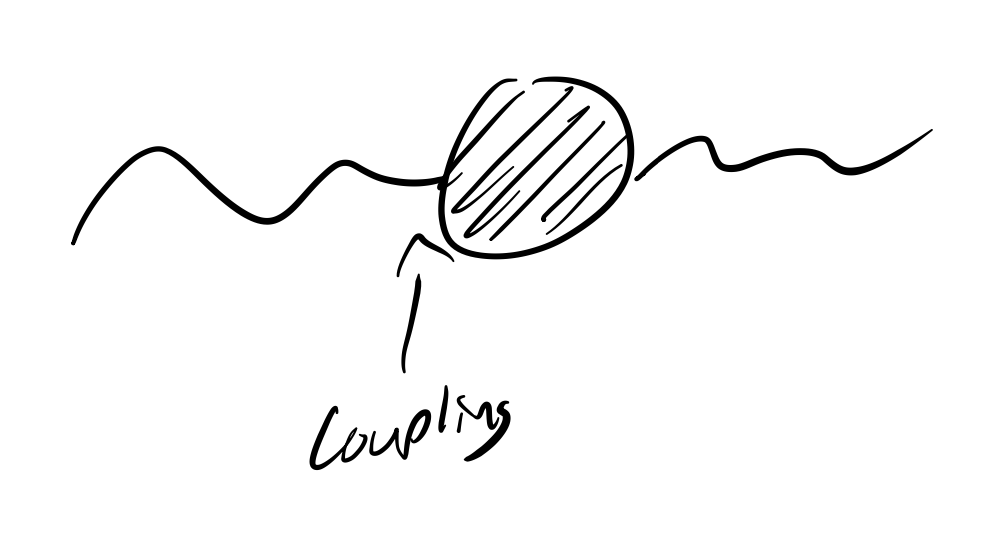
\includegraphics[scale=0.5]{Images/lec32p1.png}
\end{center}

This current is conserved when the EoMs are satisfied, so calling the irreducible two-point function of this $\Pi_{\mu\nu}(p^2)$m we know that $p^\mu \Pi_{\mu\nu}(p^2) = 0$. In the textbook there is a complicated functional derivation of this (one of a more general set of identities known as Ward-Takahashi identities). Note that we then have:
\begin{equation}
    \Delta_{\mu\nu}^{-1} = ip^2\left(\eta_{\mu\nu} - \frac{p_\mu p_\nu}{p^2}\right) + i \xi \frac{p_\mu p_\nu}{p^2}
\end{equation}
So if this is the inverse of the two point function of the free photon, then the inverse of the two point function of the interacting photon is:
\begin{equation}
    D^{-1}_{\mu\nu} = \Delta^{-1}_{\mu\nu} + i\Pi_{\mu\nu}
\end{equation} 
the current is conserved even if we add a mass term:
\begin{equation}
    \Delta_{\mu\nu}^{-1} = ip^2\left(\eta_{\mu\nu} - \frac{p_\mu p_\nu}{p^2}\right) + i \xi \frac{p_\mu p_\nu}{p^2} + i\kappa^2 \eta_{\mu\nu}
\end{equation}
and even this one does not get corrected. This has to do with current conservation, nothing to do with Gauge invariance really.

Say we now calculate:

\begin{center}
    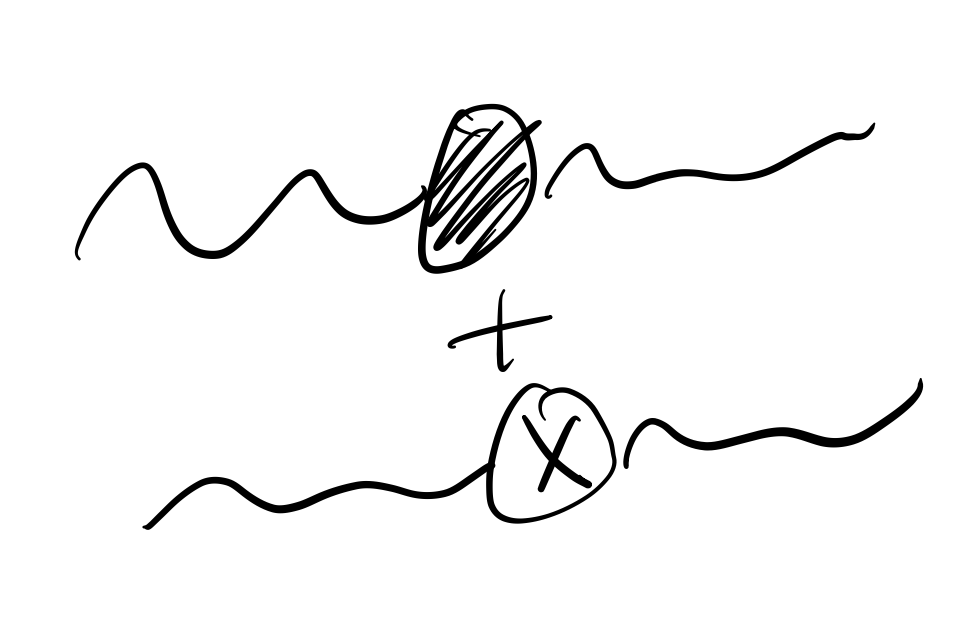
\includegraphics[scale=0.5]{Images/lec32p2.png}
\end{center}

The result is:
\begin{equation}
    \Pi_{\mu\nu} = i(k^2\eta_{\mu\nu} - k_\mu k_\nu) \frac{e^2}{2\pi^2}\int_0^1 d\alpha \alpha(1-\alpha)\ln(1 + \alpha(1-\alpha)\frac{k^2}{m^2})
\end{equation}
There was a singularity, but we adjusted the counter-term to cancel the singularity. The correction vanishes as $k^2 \to 0$, so the pole in the two-point function remains at $k^2 = 0$. The counter-term has been adjusted so that the residue is just as it was for the free-photon (the ``on-shell'' subtraction scheme). We could grind through the calculation, but we did it already in class for the scalar field theory, and you have the electron calculation for HW. So let's not go through it here.

\subsection{Recovering Coulomb from QED}
Electrodynamics is a very interesting subject - you start studying it in high school in an elementary fashion, then in undergraduate the classical version is studied, and then in this class we learn it is actually a quantum field theory. And everything we have done so far has just been a classical approximation to the QFT. We have taken the photon field and written it as some classical field:
\begin{equation}
    \mathcal{A}_\mu(x) = A_\mu(x) + a_\mu(x)
\end{equation}
where the first term is a classical field and the second term is the quantum operator (analogously so how we wrote the bose field operator). If the Bose gas was weakly coupled then things were basically classical, with the quantum part providing small corrections. In a sense, that is what we are doing here with QED; we are learning how to include the operator term, when we already know a lot about how the classical EM fields work.

So, let's try to include these QED corrections into our classical understanding of electrodynamics! Imagine we have a charge distribution $\rho(\v{x})$. This has a Coulomb energy - the work required to assemble the distribution against the Coulomb force. This has the expression:
\begin{equation}
    E = \frac{1}{2}\int d^3x d^3y \rho(\v{x})\frac{1}{4\pi\abs{\v{x} - \v{y}}}\rho(\v{y})
\end{equation}
This must be a pretty good approximation, because all of the electrical engineers in the world seem to be doing pretty well, without knowing anything about QED. But, let's try to find what the corrections are, anyway. How would we incorporate a charge density $\rho$ into the quantum field theory? Well, we already have the coupling:
\begin{equation}
    A_\mu \bar{\psi}\gamma^\mu \psi
\end{equation}
well the $\bar{\psi}\gamma^\mu \psi$ is just the $\psi^\dag \psi$, the number operator for the Fermion field, which gives a charge when we multiply by a quantum of electric charge $e$. So why not just add it there?  Further, $\v{x}$ is time-independent, so why don't we just think about this as the interaction Hamiltonian:
\begin{equation}
    H_{int} = \int d^3x A_0(\v{x})\rho(\v{x})
\end{equation}
The shift in energy of the QED vacuum $\ket{0}$ when we add this bit to the Hamiltonian (to first-order in perturbation theory) is:
\begin{equation}
    E^{(1)} = \bra{0}H_{int}\ket{0}
\end{equation}
Here we can make $\rho(\v{x})$ small enough such that the correction to linear order is the only important one. This expectation value is equal to zero:
\begin{equation}
    E^{(1)} = \bra{0}H_{int}\ket{0} = 0
\end{equation}
because $H_{int}$ is linear in $A_\mu$ and the expectation value of $A$ is zero. So, I guess this means that we have to be a little more sophisticated and go to second order perturbation theory. There, we have:
\begin{equation}
    E^{(2)} = -\bra{0}H_{int}\frac{1}{H - E_0}H_{int}\ket{0}
\end{equation}
with $E_0$ the vacuum energy and $H$ the vacuum Hamiltonian.
This is better because it is quadratic in $\rho$ and the classical energy is also quadratic in $\rho$, so this might be what we expected anyway. We've done this kind of perturbation theory before for rough arguments (and we may have discouraged it a bit), but here if it is all we want to do then it is not too daunting to evaluate.

How do we develop this? In a sense when we do this perturbation theory in the Schrodinger picture, we can just set the time equal to zero (otherwise the interaction Hamiltonian does not commute with the other Hamiltonian, and the perturbation becomes time-dependent). We want to play with this formula a little bit, and one thing we can do is to rewrite it as follows:

\begin{equation}
    E^{(2)} = -i\int_0^\infty dt \bra{0}H_{int}e^{-it(H - E_0 - i\e)}H_{int}\ket{0}
\end{equation}
Using this to conjugate, knowing that $E_0$ is the vacuum energy:
\begin{equation}
    E^{(2)} = -i\int_0^\infty dt \bra{0}H_{int}(t)H_{int}(0)\ket{0}
\end{equation}
so substituting in what the interaction Hamiltonian actually is:
\begin{equation}
    E^{(2)} = -i\int_0^\infty dt \int d^3x \int d^3y \rho(\v{x})\rho(\v{y})\bra{0}A_0(\v{x}, t)A_0(\v{y}, 0)\ket{0}
\end{equation}
%And now, we can turn this to an integral over an infinite domain of $t$ by multiplying by a half and making the operators time ordered. 
Remember that a two point function like we see above is only dependent on the difference between the two coordinates. So, I can write it as a half of what is written here plus a half of $A_0(\v{x}, -t)A_0(\v{y}, 0)$. We can then write the integral over an infinite time domain:
\begin{equation}
    E^{(2)} = -\frac{i}{2}\int_{-\infty}^\infty dt \int d^3x d^3y \rho(\v{x})\rho(\v{y})\bra{0}TA_0(\v{x}, t)A_0(\v{y}, 0)\ket{0}
\end{equation}
The correction to the Coulomb interaction here is:
\begin{equation}
    V(\abs{\v{x} - \v{y}}) = -i\int_{-\infty}^\infty dt D_{00}(\v{x}, t; \v{y}, 0)
\end{equation}
so the statement is that the time-time component integrated over all times (projected to zero frequency in momentum space) is not just the corrected Coulomb interaction, but the full prediction of what the Coulomb energy is; classical and quantum included! Is this reasonable? Let us go to momentum space:
\begin{equation}
    V(\v{k}) = -iD_{00}(k^0 = 0, \v{k}) = -i\Delta_{00}(k^0 = 0, \v{k}) + \ldots
\end{equation}
At order $e = 0$, we must have the classical energy, so $\Delta_{00}$ should correspond to the classical energy. Is this right? Recall:
\begin{equation}
    \Delta_{\mu\nu} = \frac{-i\eta_{\mu\nu}}{k^2} + \frac{ik_\mu k_\nu}{(k^2)^2} + \xi\ldots
\end{equation}
Talking the zero/zero component, we see that the second and third terms cancel. So result number 1 - it is independent of the Gauge fixing parameter $\xi$! This is good. We then have:
\begin{equation}
    \Delta_{00} = \frac{i}{\v{k}^2}
\end{equation}
So, in terms of the inverse fourier transform:
\begin{equation}
    V(\abs{\v{x} - \v{y}}) . = \int \frac{d^3k}{(2\pi)^3}e^{ik(x - y)}\left(\frac{1}{\v{k}^2} + \ldots \right)
\end{equation}
and of course, the fourier transform of $\frac{1}{\v{k}^2}$ is just:
\begin{equation}
    \frac{1}{4\pi\abs{\v{x} - \v{y}}}
\end{equation}
so we recover the Coulomb interaction, which is great for the correctness of QED! Now let's see if we can find the corrections.

\subsection{Corrections to Coulomb from QED}
Looking at the correction to order $e^2$, we have:
\begin{equation}
    V(\abs{\v{x} - \v{y}}) = \int \frac{d^3k}{(2\pi)^3}e^{ik(x - y)}\left(\frac{1}{\v{k}^2(1 - \frac{e^2}{2\pi^2}\int_0^1 d\alpha \alpha (1 - \alpha \ln(1 + \frac{\alpha(1-\alpha)\v{k}^2}{m^2})))}\right)
\end{equation}
Taylor expanding in $\v{k}^2$, we are able to do the integrals. When we do this, we get something that looks like:
\begin{equation}
    V(\abs{\v{x} - \v{y}}) = \int \frac{d^3k}{(2\pi)^3}e^{ik(x - y)}\left(\frac{1}{\v{k}^2} + \frac{e^2}{60\pi^2}\frac{1}{m^2} + \ldots\right)
\end{equation}
i.e. a tiny repulsive constant. So, the good old Coloumb interaction is good to $0.1\%$ or so. But in any case, there is such a term, and when we do the Fourier transform, we have a contact interaction:
\begin{equation}
    V(\abs{\v{x} - \v{y}}) \sim \frac{1}{4\pi\abs{\v{x} - \v{y}}} + \frac{e^2}{60\pi^2}\frac{1}{m^2}\delta^3(\v{x} - \v{y})
\end{equation}
which is called the Uelling term. It is more or less known to be needed. For example in the hydrogen atom if one corrects the Coloumb interaction by this, this only shifts the s-wave states by $\sim 50\si{MHz}$. When $\v{k}$ gets small, the correction vanishes, but when $\v{k}$ gets large the coupling appears to get larger (leads to a correction to Coulomb of about $\sim 5\%$). This formula can be improved significantly by considering the renormalization group. One could apply the RG group idea to study this at different momenta. This would basically replace $e^2$ by the running coupling constant, but unfortunately $e^2$ itself runs to strong coupling at high-energy, so it does not fix up the fact that this grows at high energy. In fact the RG resummation grows even faster at high energy (but RG does make the low-energy result more reliable).

This calculation is a good example of using the things we have learned so far - to recover (and correct) the Coulomb interaction we only needed to do a one-loop integral!

\subsection{Vertex Corrections}
The above calculation was quite straightforwards. Unfortunately, going anywhere beyond this adds some layers of technical difficulty. But let us discuss just a little about what one does to calculate the vertex function. This all came from a two-point function, the simplest correlation function one could think of computing. There is also a three-point function which in a sense contains the quantum corrections to the interaction vertex. We consider the irreducible correlation function:
\begin{equation}
    \Gamma_{I\mu ab}(q, p, p') = \bra{0}TA_\mu(x)\psi_a(y)\bar{\psi}_b(z)\ket{0}
\end{equation}
calculating corrections to this can tell us corrections to photon-electron interactions.To leading order, we had:
\begin{equation}
    \Gamma_{I\mu ab}(q, p, p') = -ie[\gamma_\mu]_{ab}
\end{equation}
i.e. just the vertex. It's of interest to calculate the corrections to this. In terms of Feynman diagrams, this is not very hard:

\begin{center}
    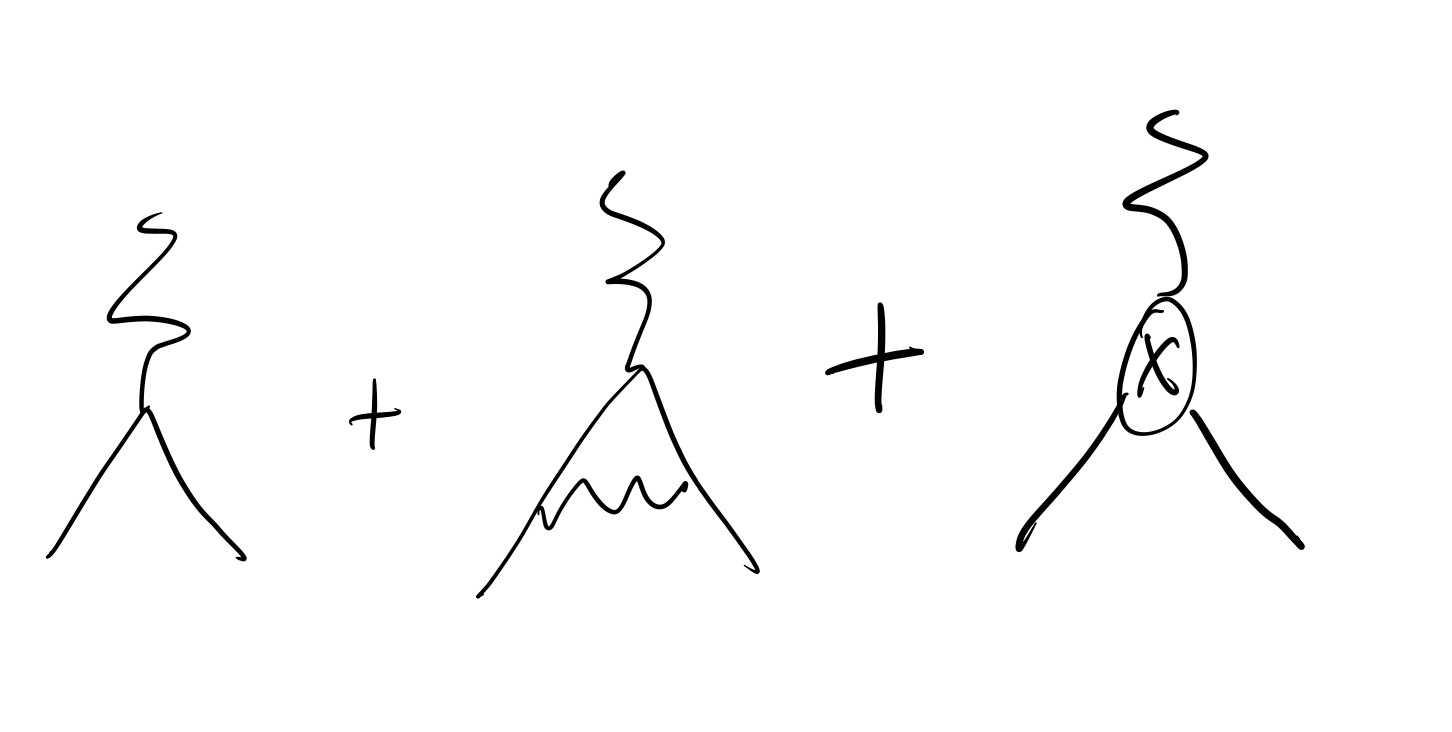
\includegraphics[scale=0.5]{Images/lec32p3.png}
\end{center}

But unfortunately the simplicity starts the second we write down the Feynman integral and try to solve it. This can be done, using more or less the same techniques that we know. One thing that does happen here that we have not encountered so far is an infrared divergence. This occurs when you want to calculate an S-matrix element using an LSZ like formula. We amputate the legs, then put the external momenta on-shell - but this is not kinematically possible. On-shell conditions and energy/momentum conservation are not compatible, as else photons would be unstable and could decay into an electron/positron pair. So, one uses the second central diagram as a subprocess of something else. 

When we do this, we get:
\begin{center}
    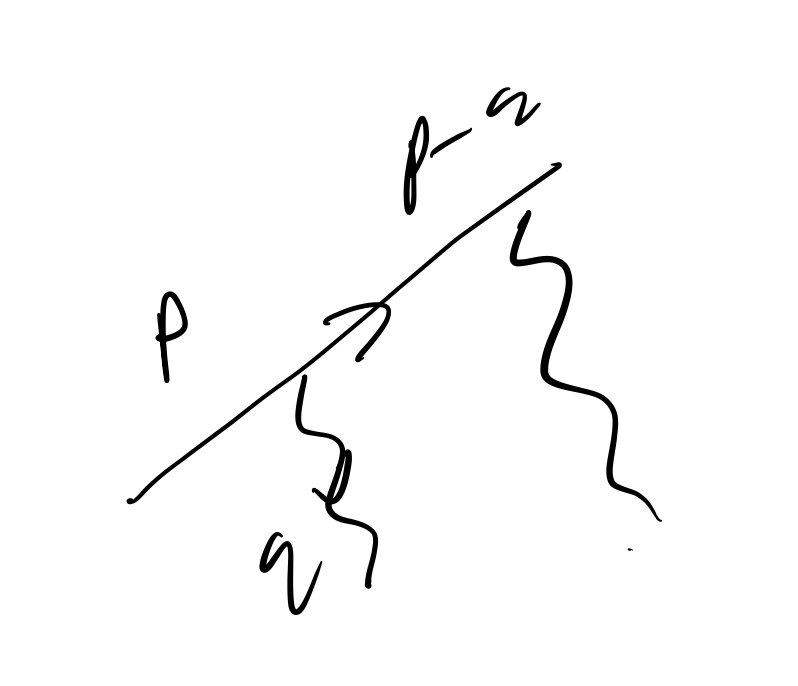
\includegraphics[scale=0.5]{Images/lec32p4.png}
\end{center}
With propogator:
\begin{equation}
    \bar{\psi}(p)\gamma^\mu \frac{i(\slashed{p} - \slashed{q}) - m}{(p - q)^2 + m^2}
\end{equation}
Which simplifies:
\begin{equation}
    \bar{\psi}(p)\frac{\gamma^\mu}{-2\v{p} \cdot \v{q}}
\end{equation}
If we do the same thing on the other side of the diagram, we get:
\begin{equation}
    \frac{\gamma^\mu}{2\v{p}' \cdot \v{q}}\psi(p')
\end{equation}
we then multiply by the photon propogator $\frac{1}{q^2}$ and integrate over four-momenta $p$. We know have some divergences. There are divergences at large $q$, but this is fixed by renormalization. We also have infrared singularities, at small $q$ however - renormalization does not fix this. This is a still developing area. They occur when we enforce the on-shell conditions, and the problem is in a sense that the $\frac{1}{q^2}$ is a long-range interaction, and some of the assumptions that go into the S-matrix (the particles scatter and become free of each other) are wrong. You can see this in NRQM where the cross section for Coulomb scattering has a logarithmic divergence. This is a very subtle problem requiring extra interpretation.

A comment on quantum gravity - If you treat gravity as an effective field theory, where we linearize around flat space, it is not renormalizable (We need an infinite number of counterterms, but the number of counterterms for a given order are finite). Moreover the counterterms do not affect the low-energy processes. So if you make an agreement to do quantum gravity in low-energy limit only, things sort of work out. However you still get infrared divergences, roughly coming from the $\frac{1}{r}$ gravitational potential. There has been some discussion about this for the black hole information paradox - perhaps it is resolved by these long-range interactions. If we throw our QFT textbook into a black hole, perhaps we can recover the information from the gravitons emitted. The solution to this infrared problem is not super well-understood.

There is actually some better news here. If we take the matrix element we were talking about:
\begin{equation}
    \bar{\psi}_a(p)\Gamma^\mu_{ab}(a, p, p')\psi_b(p')
\end{equation}
with the $p$s on shell, this has a decomposition into things known as form factors:
\begin{equation}
    \bar{\psi}_a(p)\Gamma^\mu_{ab}(a, p, p')\psi_b(p') = F_1(q^2)\bar{\psi}(p)\gamma^\mu \psi(p') + F_2(q^2)\bar{\psi}(p)\Sigma^{\mu\nu}\psi(p') (p - p')^\nu
\end{equation}
just by symmetry we can show that this has this form. This matrix element is a function of two functions, each of which is a function of just one variable. $F_1$ is known as the electric form factor and $F_2$ the magnetic one. It turns out that (at least at the one loop level) all of the difficulties lie in the electric form factor. The UV and IR divergences, and the counterterms are all in $F_1$. $F_2$ is beautifully finite, and can be calculated. What's more, this tells us how electrons interact with magnetic fields, and how quantum corrections change this. It is not particularly obvious from this relativistic form, and it shouldn't be because we can turn magnetic fields into electric fields via a Lorentz boost, but if we put the electron at rest (or nearly at rest) then the first term contains the charge of the electron, and the second term contains a correction to its magnetic moment. And so by computing $F_2$, we can compute corrections to the magnetic moment. And $F_2$ is something that has been computed to 10 decimal places. And it agrees to experiment to 8 decimal places (in fact the computation has outstripped the experiment). We see a correction to the $g$-factor of the electron $\frac{1}{2}$ of $0.1\%$, and corrections to this correction are exceedingly small. The individual Feynman diagrams of four-loops don't look particularly complex:

\begin{center}
    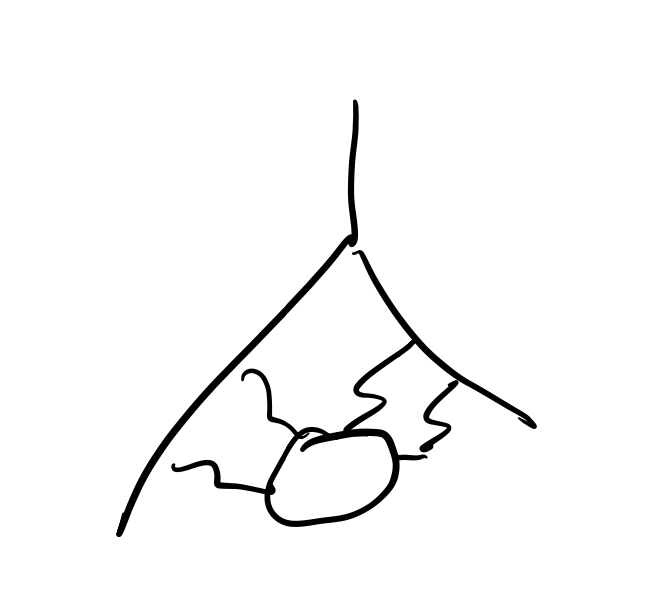
\includegraphics[scale=0.5]{Images/lec32p5.png}
\end{center}

But if you are going to do these computations, don't start with Wick's theorem. Use google to find some software, or write a computational routines yourself to write down the feynman integral and simplify it. There are often beautiful simplifications/cancellations which are not well understood. For example, 
\begin{center}
    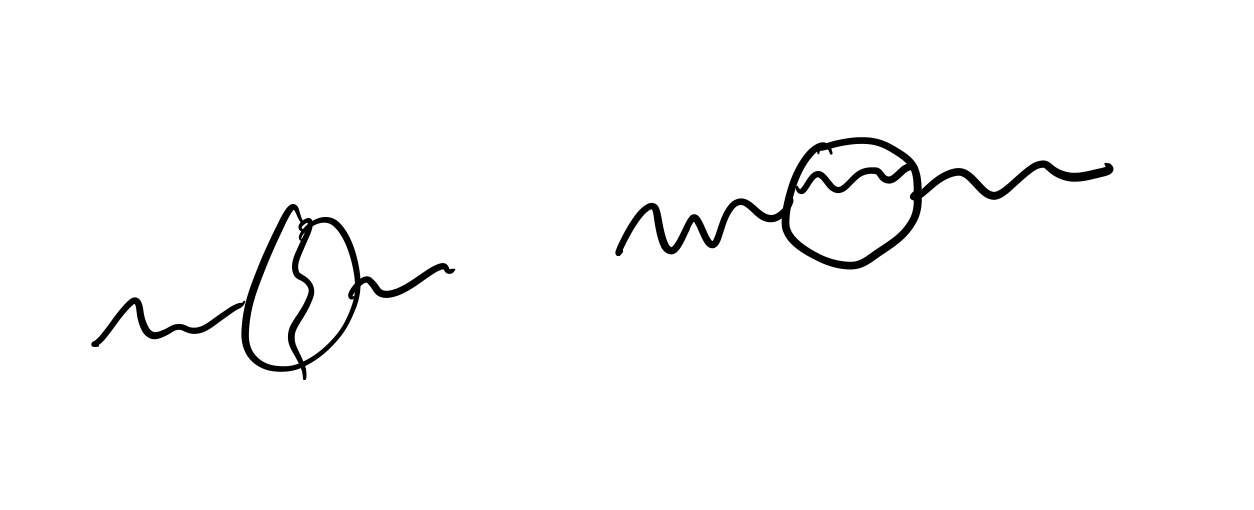
\includegraphics[scale=0.5]{Images/lec32p6.png}
\end{center}
almost cancel. In any case - for any long computation, use computers!

This is as far as we can go for this course! I encourage you to study it more - in this course we really only get to the beginning of things.